\section{Deadlock recovery}
\label{exp:deadlock}
MultiChain can run during normal operation into a situation
where two peers are both waiting on each other.
This could resulting in a deadlock.
This situation was encountered during experimentation
and the experiment shows MultiChain correctly recovering from this situation.

In the experiment a 100 megabyte file was downloaded anonymously with 2 hops.
Anonymously downloading is decribed more in the thesis report of R. Ruigrok\cite{ruigrok-anonymous}.
There are 2 Triblers instances with exit functionality and 18 instances without exit functionality.
All instances are run locally on one machine.
The instances are run in parallel,
so the fact that all instances are run on a single machine does not cause the deadlock to occur.
There is no packetloss in this experiment.

The corresponding graph of all the MultiChains of the experiment can be seen in Figure \ref{fig:deadlock-double}.
In this graph the blocks are depicted as nodes and the previous hash pointers are edges in the graph.
The nodes have added colouring to indicate extra meaning.
Green nodes are a first block in a MultiChain of a peer.
Blue nodes are a sequential block between the same previous peers.
Red nodes are half-signed blocks.

The potential scenario of two peers both waiting can be seen multiple times in the graph and are encircled.
The scenario generates a half-signed block at both peers.
Usually the peers continue collaboration and this continuation of a sequence can be seen in subsequent blocks.
In the graph a more complicated scenario can also be seen where multiple peers timeout between each other.

\begin{figure}
	\centerline{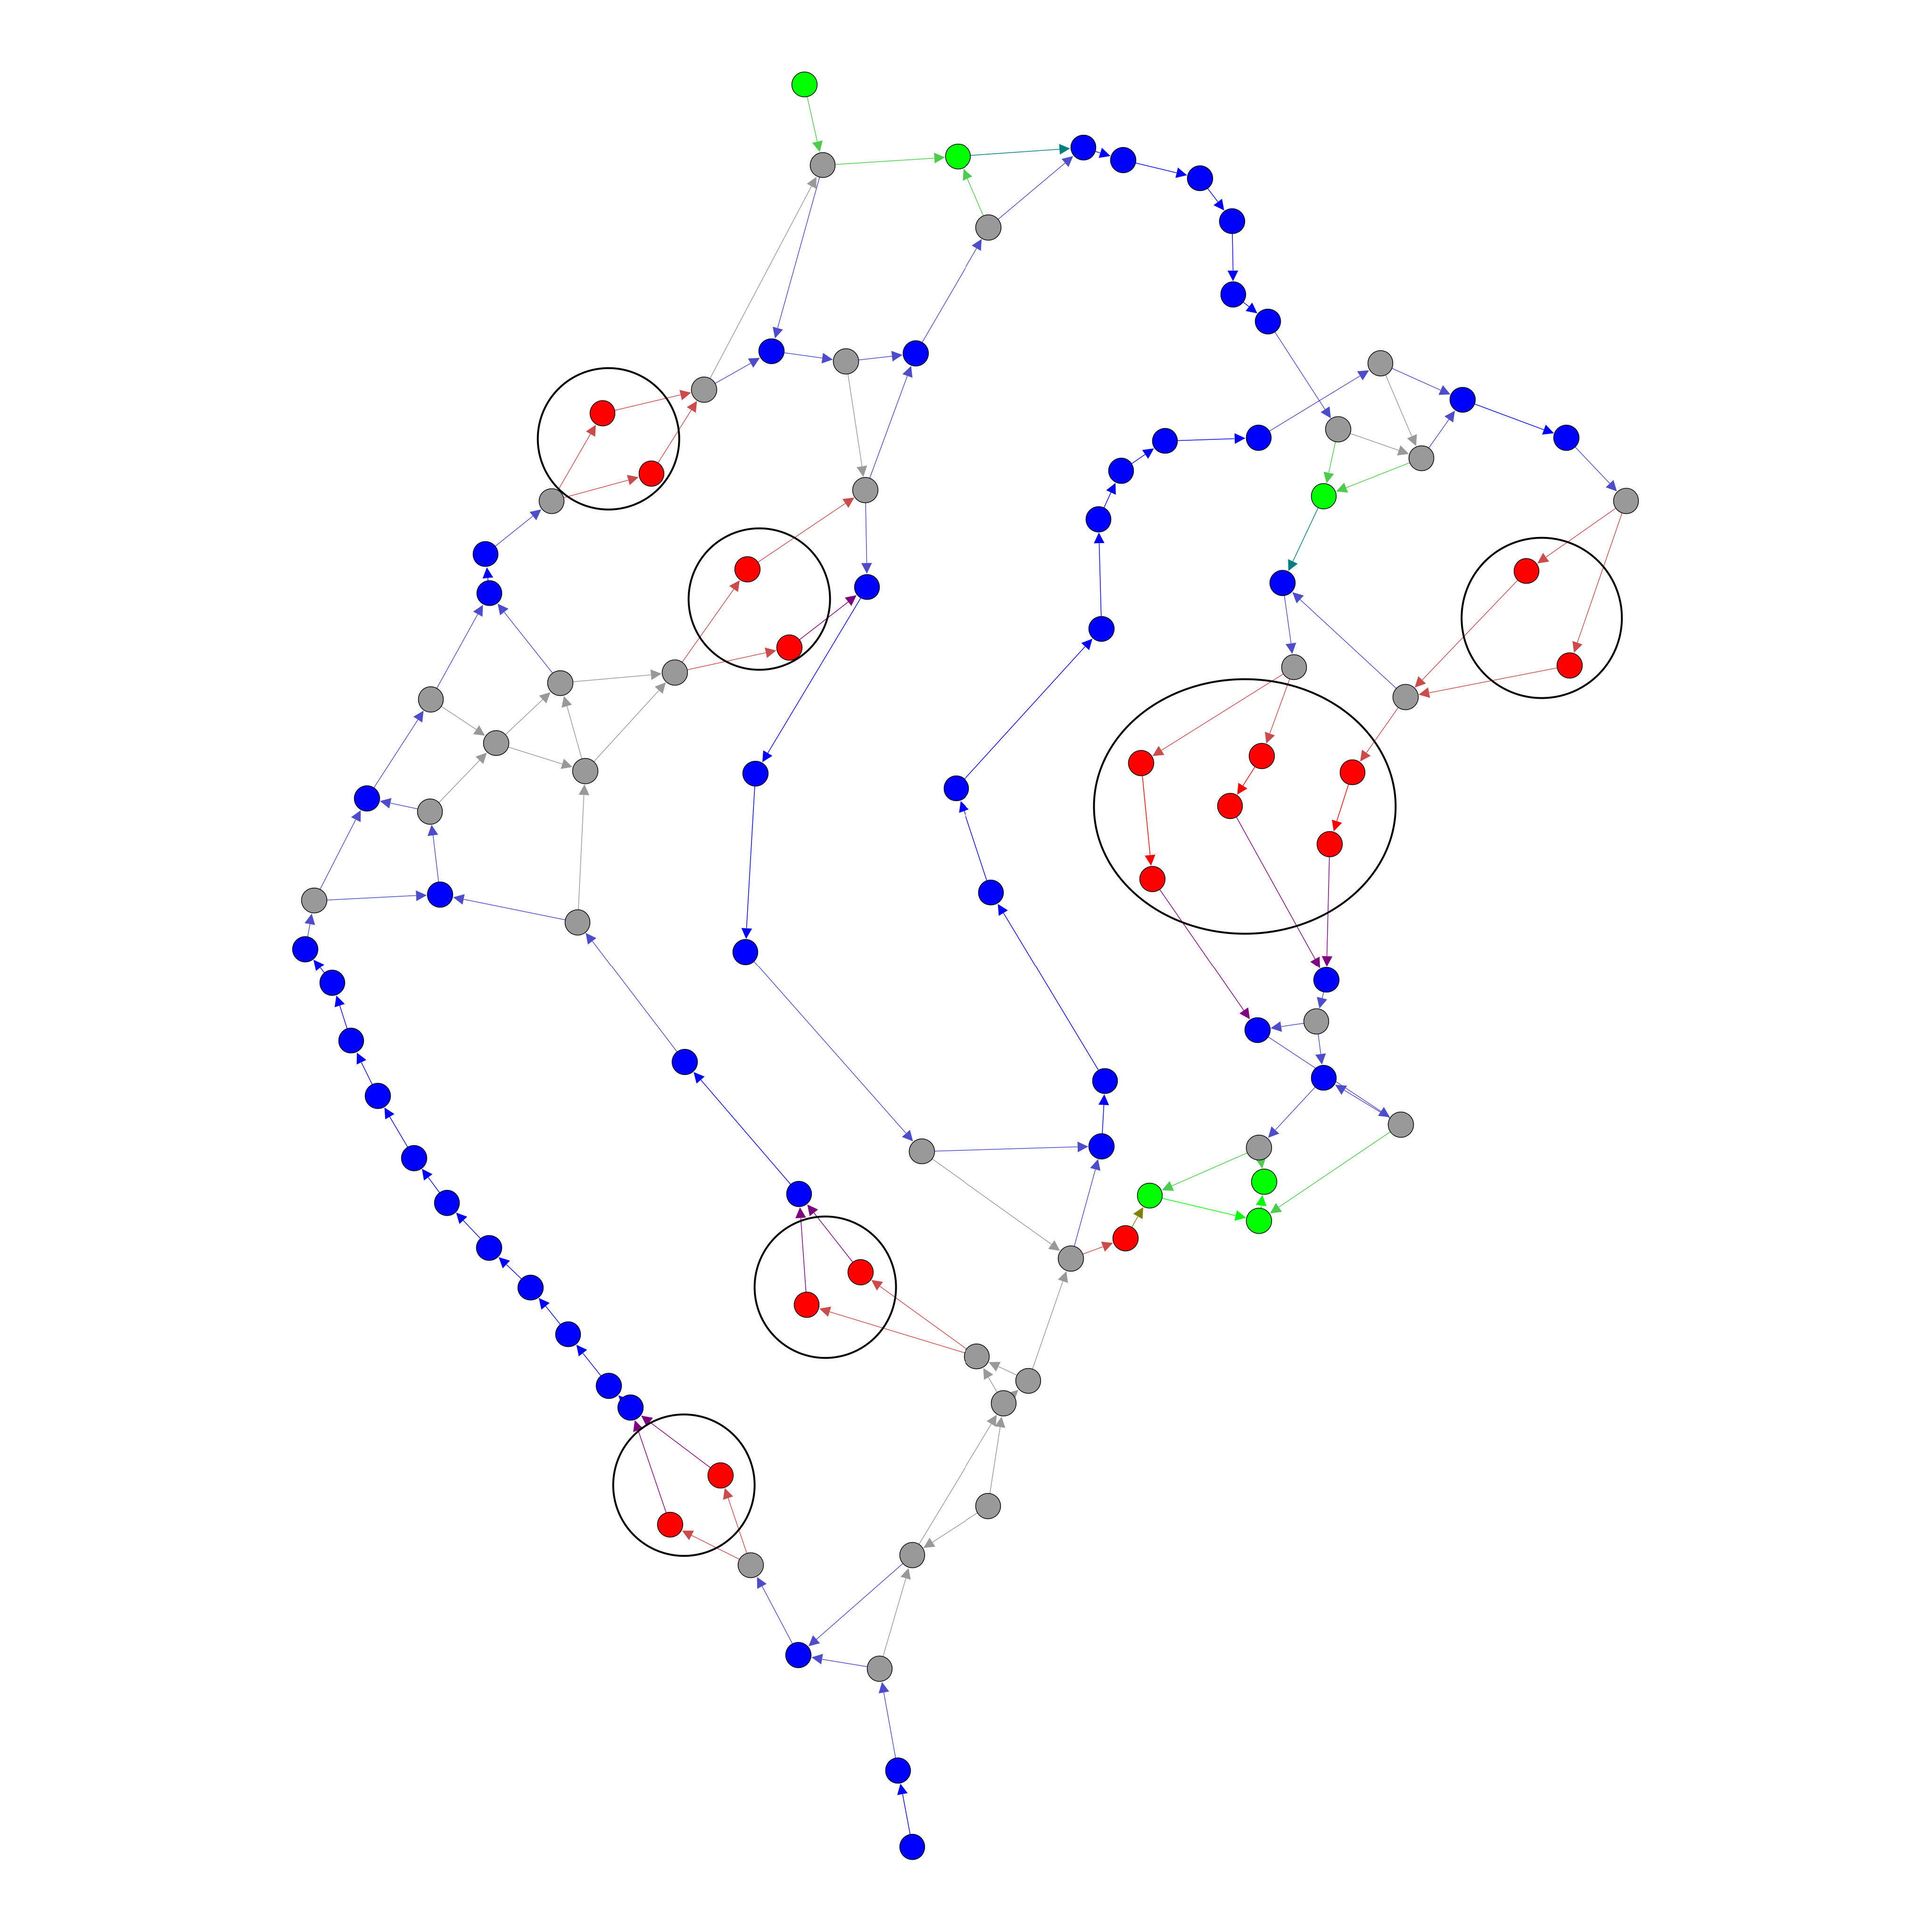
\includegraphics[scale=0.0375, bb= 0 0 4098 4098]{experimentation/deadlock/deadlock.png}}
	\caption{Potential deadlocks in MultiChain.}
	\label{fig:deadlock-double}
\end{figure}


\todo{Move to design}
When MultiChain has a pending signature request,
then it itself will not respond to incoming signature requests from other peers.
These peers themselves will also not respond, because they are not responding to requests for the same reason.
During seeding the seeder will mostly initiate signature requests to the downloader,
but the downloader will have some signature requests for metadata that he sents to the seeder.
These signature requests can be sent in such away that both sent the request before the other receives it.
Both peers are now waiting for the other to respond to the signature request and
will not answer the other resulting in a potential deadlock.
This deadlock can occur between two peers,
but can be expanded into a multiple of peers where each peer waits for another peer in a cycle.

MultiChain prevents this deadlock to occur
by allowing a transaction to fail as explained in section \ref{des:halfsigned}.
If MultiChain gets into this potential deadlock one of the peers will eventually time out of their own signature request
and process the incoming request.
The deadlock is recovered and both peers can continue operation.
